\chapter{Discussion}

\section{Challenges to Learning}

  \subsection{Learning and Inference Domain Mismatch}
  One challenge present in this study is the mismatch between the training data and the test data. The training data is inherently not beamformable into images as they are simulated point target responses rather than complete scan or simulated targets. Our evaluation dataset, including the phantom dataset and the \textit{in vivo} dataset are of specific targets and are beamformable into images.

  \subsection{Training Objective Mismatch}
  Another challenge to solving the denoising task is a mismatch between the machine learning domain and the inference domain. In our task, the training and validation in the machine learning process is in the STFT domain; the machine learning learning objective is minimizing the mean-squared-error (MSE) or Smooth Mean Absolute Error (SmoothL1) loss between the simulated STFT input and the simulated STFT target signals. However, the inference domain is in the image domain. We conduct model selection not by their loss curves, but by the beamformed image metrics and the qualitative assessment of resulting images. In other words, loss is not correlated with model performance.

  % TODO: Is this necessary
  % \subsection{Data Modes}
  % The data has three modes. We are having the neural network to learn to 1. distinguish them, and 2. output values.


% \section{CNR as a Function of Network Weights}
% Compared to the earlier LeNet-like and AlexNet-like architectures which feature both convolutional layers and fully-connected ones, the FCNs do not perform as well even though they still improve upon the benchmark DAS results. I investigate two possible reasons. First of all, the decrease in performance could be due to the decrease in the total number of weights. In other words, the CNR could be a function of the total number of weights in the model. The number of weights for the best-performing FCN is 1.64E4, which lower than that of the best-performing LeNet at 1.33E5, and more so compared with the best-performing MLP with 4.60E6. % To study this, we vary the number of convolutional layers in the model to increase the number of kernels and the number of weights in the FCN, respectively.


\section{The Role of Convolution}

\section{The Receptive Field of Convolution}
The convolution operation is inherently recursive. For an output element of a convolutional layer, not only does it depend on the input to its own layer, but it is also an indirect product of any previous convolutional layer if the layer input is a convolutional output. The theoretical receptive field (RF) describes the number of input elements that ultimately map to the final output. Conceptually, if the size of the RF approximates the size of the input, the network can be thought of as approaximating an MLP because in both elements, every output element theoretically depends on each input element. In other words, if there exists a performance gap between FCNs with full convolutional support and those without, then the convolution operation is unlikely to learn better than full connections.

The size is the RF is recursively defined for each convolutional layer as \cite{luo2016understanding}

$$
rf_size_{0} = 1
rf_size_{i} = rf_size_{i-1} + (kernel\_size - 1) * jump_{i-1}
$$
, where
$$
jump_{0} = 1
jump_{i} = jump_{i-1} * stride
$$

In other words, the size of the receptive field in relation to the input is a function of the kernel size and the stride of each layer as well as the number of (convolutional) layers. Furthermore, the upsampling operation used in FCNs does not affect the size of the RF because the recursive dependency remains unaffected.

The fact that FCNs do not outperform MLPs but improves upon the DAS benchmark could be due to the fact that convolutions may be approximating full connections by having a large receptive field to cover most of or all of the input. In order to test this hypothesis, we designed two studies.

\subsection{CNR as a Function of Convolutional Kernel Size}
The first mechanism for enlarging the RF is by increasing the kernel size. To investigate this potential effect, we used the existing FCN-4 architecture, only to vary the size of the kernel between 3 and 65 (and padding). All four convolutional layers share the same kernel size (but not the same padding size so as to ensure output resolution). In order to create a comparison between FCNs and MLPs, we concatenated the real and imaginary data as a flat list. The model search process undersamples larger kernel sizes due to an increased difficulty of ensuring output resolution at larger kernel sizes. However, Figure \ref{fig:cnr_vs_kernel_size} suggests that models with a kernel size of 9 or above dramatically outperform those under 9, with 15 producing the top-performing model (on average).

% For example, for a 1D input of length 130, a convolutional kernel size of 130 would not be able to slide across the input (without padding), but a smaller kernel of length 5 would be able to slide 125 times at a stride of 1. The former caes is no different from a full connection.
\begin{figure}[htbp]
  \centerline{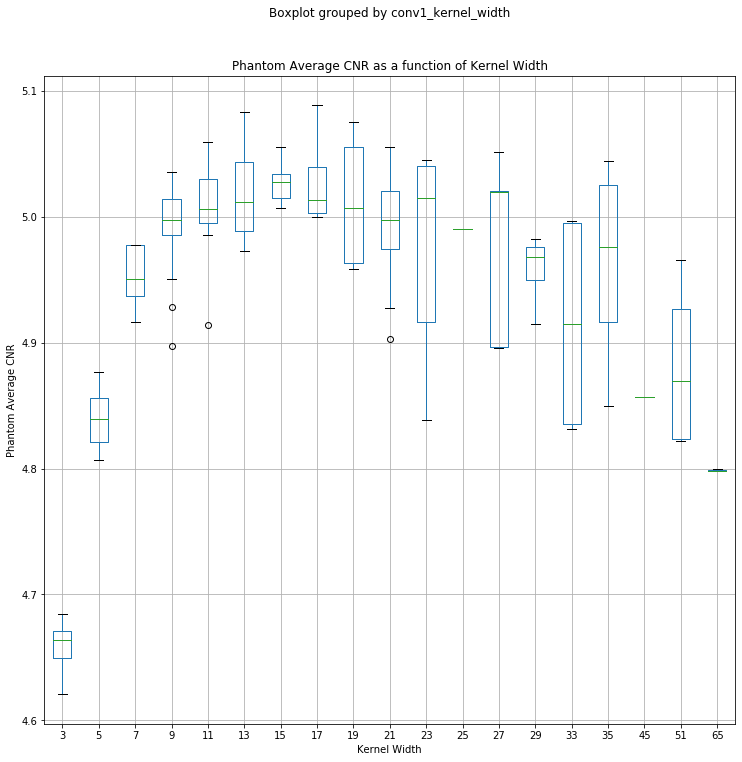
\includegraphics[width=85mm,scale=0.5]{cnr_vs_kernel_size.png}}
  \caption{Phantom average CNR as a function of convolutional kernel size, FCN-4}
  \label{fig:cnr_vs_kernel_size}
\end{figure}

\begin{figure}[htbp]
  \centerline{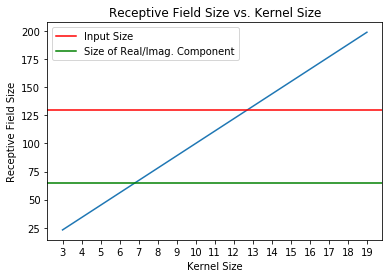
\includegraphics[width=85mm,scale=0.5]{rf_size_vs_kernel_size.png}}
  \caption{Phantom average CNR as a function of convolutional kernel size, FCN-4}
  \label{fig:rf_size_vs_kernel_size}
\end{figure}


An examination of the RF's growth pattern as a function of kernel size for the FCN-4 architecture (Figure \ref{fig:rf_size_vs_kernel_size} shows that kernel sizes 9 and 15 are both two sizes above the intersection with the real/imaginary component size and the input size, respectively. In other words, for the model whose kernel size is 9, a real output maps to all real inputs, and an imaginary output maps to all imaginary inputs; for the model with a kernel size of 15, all outputs map to all inputs. In both cases, the complex-component/full convolution support (that is, the full coverage of the RF over the input) is achieved before the final layer. It appears that having component support dramatically improves training, gains from having all input support are relatively modest. Further increases in kernel size does not offer additional benefits.



\subsection{CNR as a Function of The Number of Convolutional Layers}
Because the RF also depends on the number of convolutional layers, I further investigate my hypothesis that the convolution is approximating full connections with a large RF. For this experiment, we implemented a special architecture, FCN-N, with same padding. In other words, the input and output resolutions of each convolutional layer stay the same. In order to isolate the number of convolutional layers as the sole variable for the RF size, we only use kernel sizes smaller than 9 including 7. As before, I constrain all layers to share the same kernel size. I use a stride of 1 and same padding (which is 3 for 7). Figure \ref{fig:cnr_vs_num_layers_kernel_7} indicates that 10 layers is the approximate peak, given an incomplete sampling range over the number of layers.

\begin{figure}[htbp]
  \centerline{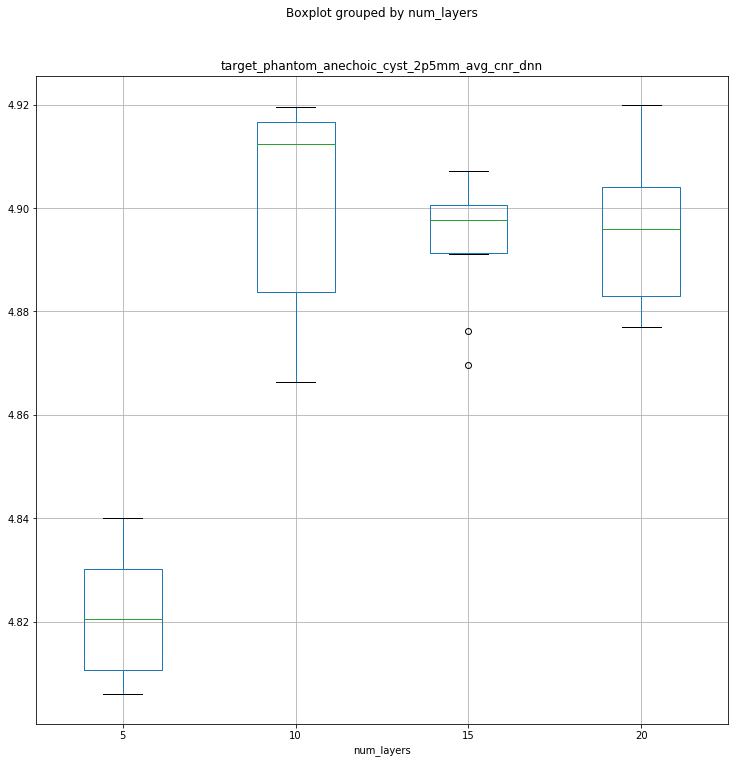
\includegraphics[width=85mm,scale=0.5]{cnr_vs_num_layers_kernel_7.png}}
  \caption{Phantom average CNR as a function of number of convolutional layers, FCN-N}
  \label{fig:cnr_vs_num_layers_kernel_7}
\end{figure}


\begin{figure}[htbp]
  \centerline{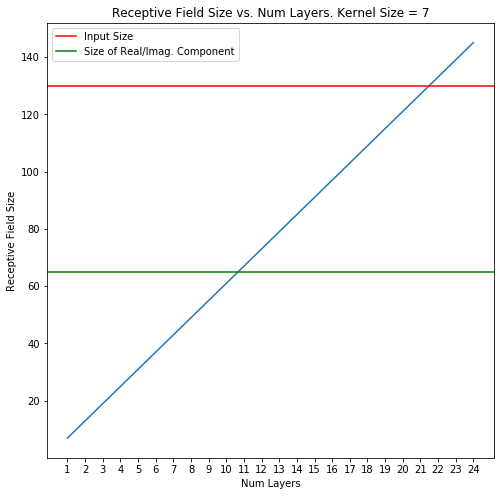
\includegraphics[width=85mm,scale=0.5]{rf_size_vs_num_layers_kernel_7.png}}
  \caption{Phantom average CNR as a function of convolutional kernel size, FCN-N}
  \label{fig:rf_size_vs_num_kernels_kernel_7}
\end{figure}

As is shown in Figure \ref{fig:rf_size_vs_num_kernels_kernel_7}, 10 is just below then number of layers needed for the RF to fully support each complex component, while I would need more layers (22 or above) to to show effects for full input support. Thus far, CNR performance appears to depend on a RF offering full compoenent support and corroborate our hypothesis that convolution alone does not extract unique features not readily learnable by MLPs.


% TODO: waiting for MLP
\section{Bottleneck and Feature Representation with MLP}
Another question remains as to why MLPs work to start with. One hypothesis is that they are overfitting by using bigger models. To test my hypothesis, I implemented bottlenecked MLPs (MLPBs) that restrict the best performing MLP (5 layers, each with 1040 nodes) to significantly reduce its middle layer (to 32, 64, 128, 256, and 512 nodes). For the 50 MLPBs trained, the phantom CNR are significantly lower than that of the best-performing MLP (Figure \ref{fig:cnr_vs_bottleneck_width}). Furthermore, none of the MLPBs outperform the reference MLP in \textit{in vivo} results. These results suggest that MLPs are not simply overfitting to the training data.
% In order to investigate whether MLPs are overfitting.
% We found that for the best models. Caveat - we only trained 50 MLPBs
\begin{figure}[htbp]
  \centerline{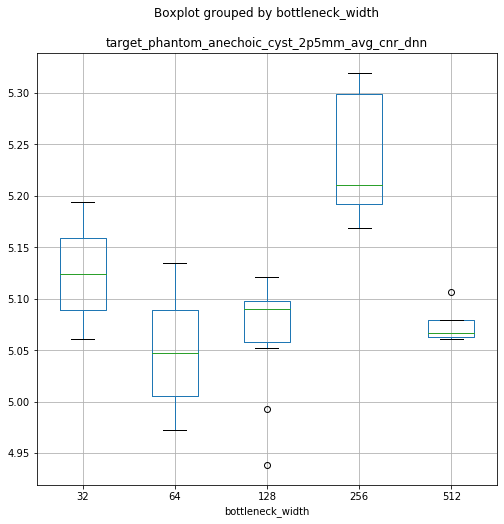
\includegraphics[width=85mm,scale=0.5]{cnr_vs_bottleneck_width.png}}
  \caption{Phantom average CNR as a function of bottleneck width, MLPB-5}
  \label{fig:cnr_vs_bottleneck_width}
\end{figure}

% % TODO: include hyperparameter analysis
% \section{CNR as a funciton of the number of weights}
% Another possibility is that the model is a that There is potential evidence to suggest that performance is a function of the number of weights.
